\subsection{Basis-set expansions and design principles}

The matrix equations in Section~\ref{sec:finite-basis-hf} assumed that the
orbital basis had already been chosen. We now examine that choice: which
functions can represent the radial and angular variations of molecular
orbitals accurately with a manageable number of coefficients?

In practical molecular calculations, each molecular orbital is expanded in a
finite set of known one-electron functions,
\begin{equation}
  \psi_p(\br)=\sum_{\mu=1}^{K}C_{\mu p}\phi_\mu(\br)
\end{equation}
The basis functions $\phi_\mu$ are fixed, whereas the coefficients $C_{\mu p}$
are determined variationally. Enlarging a nested sequence of basis spaces
increases the variational freedom and lowers, or leaves unchanged, the minimum
HF energy as the complete-basis-set (CBS) limit is approached. Basis exponents
and contraction coefficients are fixed numerical parameters, often obtained
from atomic electronic-structure calculations. Their presence does not by
itself make the method empirical; they specify the finite representation of
the otherwise ab initio problem.

Thus orbital optimization combines fixed building blocks rather than
redesigning them. Their shapes, centers, and nonlinear parameters are selected
before the SCF calculation begins and determine the available one-electron
space.

A useful basis must be accurate, compact, numerically stable, and practical.
These requirements compete: a larger and more flexible basis improves the
description of the orbitals, but increases both the computational cost and the
risk of linear dependence.

\subsubsection{The LEGO principle}

Basis-set construction follows a LEGO-like philosophy: a small collection of
well-designed building blocks is combined to describe chemically diverse
systems.
\begin{figure}[htbp]
  \centering
  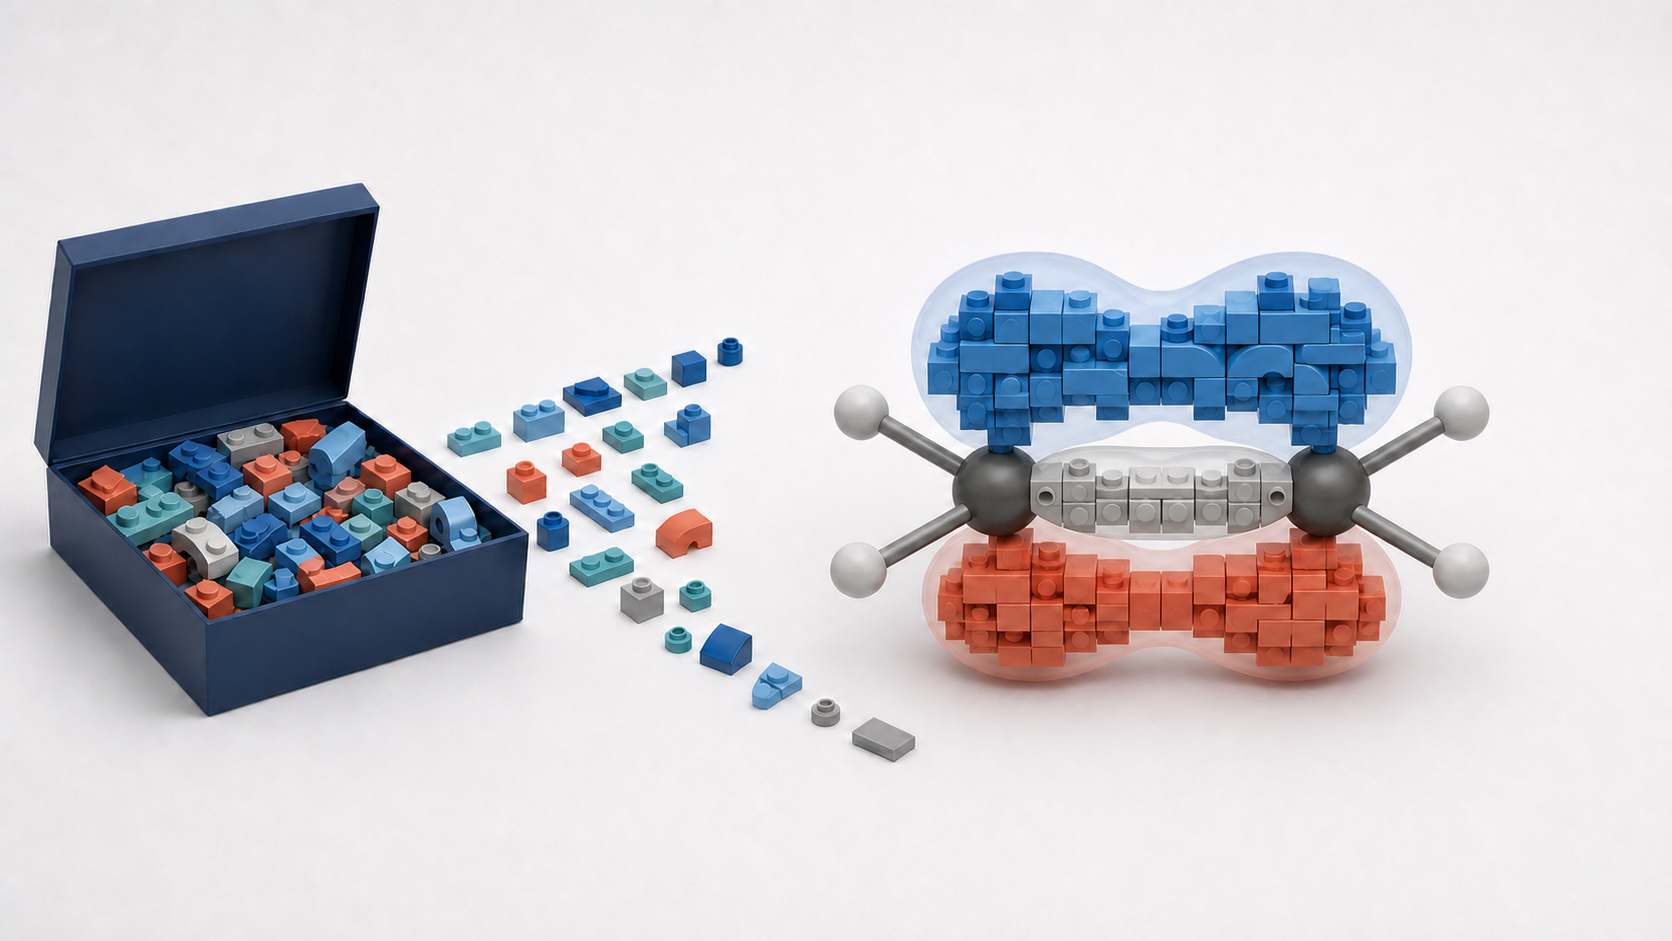
\includegraphics[width=0.62\textwidth]{lego}
  \caption{The basis functions are the elementary building blocks from which
  molecular orbitals are assembled.}
\end{figure}

The analogy also captures transferability. Atom-centered functions designed
for individual elements can be assembled in different combinations without
redesigning the basis for every molecule. The molecular environment enters
through the variational coefficients that combine these fixed building blocks.

\subsubsection{Principal families of basis functions}

Several families of one-electron functions are routinely used.
Gaussian-type orbitals (GTOs), which are proportional to
$\exp(-\alpha r^2)$, are atom centered and are the standard choice for
molecules because their multicenter integrals can be evaluated efficiently.
Here $r$ is the distance from the function's center, and $\alpha$ is a
positive Gaussian exponent.
They are used, for example, in \textsc{Orca}, \textsc{Q-Chem},
\textsc{Molcas}, \textsc{Molpro}, \textsc{PySCF}, \textsc{Psi4},
\textsc{CFOUR}, \textsc{MRCC}, and \textsc{GAMESS}.

Slater-type orbitals (STOs) are also atom centered, but are
proportional to $\exp(-\zeta r)$. Their radial form can reproduce a nuclear
cusp and an exponential long-range tail, and they are used, for example, in
\textsc{ADF}. The positive exponent $\zeta$ controls their radial extent.
By contrast,
plane waves (PWs), proportional to $\exp(\ii\bk\cdot\br)$, are
delocalized, mutually orthonormal, and naturally adapted to periodic boundary
conditions. Here $\bk$ is the wavevector and $\ii$ the imaginary unit.
Their basis size is controlled by an energy cutoff, and they are
used in \textsc{Quantum Espresso}, \textsc{VASP}, \textsc{ABINIT}, and
\textsc{CASTEP}. Finally, numerical atomic orbitals (NAOs) have
tabulated radial parts. Their compactness and flexibility make them useful in
programs such as \textsc{FHI-aims} and \textsc{SIESTA}.

\subsection{Plane-wave basis sets}

The four families balance radial accuracy, integral efficiency, periodicity,
and numerical flexibility differently. We first examine the delocalized
plane-wave representation, then return to atom-centered functions.

Plane waves are the natural one-electron functions of a translationally
invariant system. Under periodic boundary conditions, only reciprocal-lattice
wavevectors are compatible with the periodicity of the simulation cell.

In a unit cell of volume $\Omega$, a normalized plane wave is
\begin{equation}
  \phi_{\bk}(\br)=\frac{1}{\sqrt{\Omega}}\exp(\ii\bk\cdot\br)
  \qquad \abs{\bk}\leq k_\text{cut}
  \qquad E_\text{cut}=\frac{k_\text{cut}^2}{2}
\end{equation}
The reciprocal-lattice vector is indexed by three integers:
\begin{equation}
  \bk=k_1\bb_1+k_2\bb_2+k_3\bb_3
\end{equation}
where, for direct-lattice vectors $\ba_1,\ba_2,\ba_3$,
\begin{align}
  \Omega&=\ba_1\cdot(\ba_2\times\ba_3)
  &\bA&=(\ba_1,\ba_2,\ba_3)\\
  \bb_1&=2\pi\frac{\ba_2\times\ba_3}{\Omega}
  &\bb_2&=2\pi\frac{\ba_3\times\ba_1}{\Omega}
  &\bb_3&=2\pi\frac{\ba_1\times\ba_2}{\Omega}
\end{align}

The reciprocal vectors satisfy $\ba_i\cdot\bb_j=2\pi\delta_{ij}$. The energy
cutoff selects reciprocal-lattice vectors inside a sphere of radius
$k_\text{cut}$ and therefore supplies a single systematic parameter for
enlarging the basis.

The overlap integrals are diagonal:
\begin{align}
  \braket{\bk_1}{\bk_2}
  &=\frac{1}{\Omega}\int_\Omega
    \exp[-\ii\bk_1\cdot\br]\exp[\ii\bk_2\cdot\br]\dd\br\\
  &=\frac{1}{\Omega}\int_\Omega
    \exp[\ii(\bk_2-\bk_1)\cdot\br]\dd\br
  =\delta_{\bk_1\bk_2}
\end{align}
The kinetic-energy integrals are diagonal as well:
\begin{align}
  \mel{\bk_1}{-\frac12\laplacian}{\bk_2}
  &=\frac{1}{\Omega}\int_\Omega
    \exp[-\ii\bk_1\cdot\br]
    \qty(-\frac12\laplacian)\exp[\ii\bk_2\cdot\br]\dd\br\\
  &=\frac{k_2^2}{2\Omega}\int_\Omega
    \exp[\ii(\bk_2-\bk_1)\cdot\br]\dd\br
  =\frac{k_2^2}{2}\delta_{\bk_1\bk_2}
\end{align}
For the plane-wave ERI, we use the physicists' index grouping:
the first and third indices belong to electron 1, and the second
and fourth to electron 2. Its round-bracket counterpart would therefore be
$\rbraket{\bk_1\bk_3}{\bk_2\bk_4}$, rather than
$\rbraket{\bk_1\bk_2}{\bk_3\bk_4}$. The integral begins as
\begin{align}
  \braket{\bk_1\bk_2}{\bk_3\bk_4}
  &=\frac{1}{\Omega^2}\iint_\Omega
  \frac{\exp[\ii(\bk_3-\bk_1)\cdot\br_1]
        \exp[\ii(\bk_4-\bk_2)\cdot\br_2]}
       {r_{12}}\dd\br_1\dd\br_2
\end{align}
Under periodic boundary conditions, the Coulomb kernel is understood as its
periodic counterpart. With its zero Fourier component omitted, the
reciprocal-space resolution is
\begin{equation}
  v_\Omega(\br_1-\br_2)=\frac{1}{\Omega}\sum_{\bk\ne\bO}
  \frac{4\pi}{k^2}\exp[\ii\bk\cdot(\br_1-\br_2)]
\end{equation}
The $\bk=\bO$ term requires a specified electrostatic convention, for
example a neutralizing background. The symbol $r_{12}^{-1}$ in the preceding
integral represents this periodic kernel in the following calculation.
Relabeling the reciprocal summation vector $\bk\to-\bk$ gives
\begin{align}
  \braket{\bk_1\bk_2}{\bk_3\bk_4}
  &=\frac{1}{\Omega^3}\sum_{\bk\ne\bO}\frac{4\pi}{k^2}
  \iint_\Omega\exp[\ii(\bk_3-\bk_1-\bk)\cdot\br_1]
  \exp[\ii(\bk_4-\bk_2+\bk)\cdot\br_2]\dd\br_1\dd\br_2\\
  &=\frac{1}{\Omega}\sum_{\bk\ne\bO}\frac{4\pi}{k^2}
  \delta_{\bk_3-\bk_1-\bk,\bO}
  \delta_{\bk_4-\bk_2+\bk,\bO}\\
  &=\frac{4\pi}{\Omega\abs{\bk_1-\bk_3}^2}
  \delta_{\bk_1+\bk_2,\bk_3+\bk_4}
\end{align}
The Kronecker delta expresses conservation of crystal momentum.
The last expression applies when $\bk_1\ne\bk_3$. For zero momentum
transfer, the omitted zero Fourier component gives zero under the convention
used here; the fraction must not be evaluated with a zero denominator.

The simplicity of these expressions follows because differentiation and
convolution become multiplication in reciprocal space. Overlap and kinetic
energy are diagonal, while a two-electron integral survives only when the
total incoming and outgoing wavevectors are equal.

The key physical picture is that assemblies of atoms are treated as slight
distortions of free electrons. Plane waves are orthonormal and independent of
the atomic positions; naturally compatible with periodic boundary conditions;
systematically convergent through the single parameter $E_\text{cut}$; and
diagonalize the kinetic and Coulomb operators in reciprocal space. They also
permit efficient fast-Fourier-transform evaluation and have neither basis-set
superposition error nor atom-centered Pulay forces. Their limitations are
large basis sizes,
\begin{equation}
  N_\text{PW}\propto\Omega E_\text{cut}^{3/2}
\end{equation}
Core orbitals require prohibitively large cutoffs, motivating
pseudopotentials; the cost increases with supercell size; delocalized functions
provide little real-space sparsity; and the large virtual spaces make
correlated methods expensive.
Plane waves are therefore especially effective for periodic valence-electron
calculations, usually in conjunction with pseudopotentials \citep{Payne1992}.

\subsection{Slater-type and Gaussian-type orbitals}

For isolated atoms and molecules, atom-centered functions provide a compact
description by placing radial flexibility where the electronic density is
concentrated. The central choice is between radial forms that reproduce the
exact local behavior and forms that permit efficient multicenter integration.

In the following Slater- and Gaussian-type orbitals, $n$ labels the radial
form, $\ell$ and $m$ are the angular-momentum and magnetic quantum numbers,
and $Y_{\ell m}(\hat{\br})$ is a spherical harmonic evaluated in the direction
of $\br$. The Slater radial form is associated historically with screened atomic
orbitals \citep{Slater1930Orbitals}. The general forms used in the comparison are
\begin{equation}
 \phi_{\zeta n\ell m}^\text{STO}(\br)
 \propto r^{n-1}e^{-\zeta r}Y_{\ell m}(\hat{\br})
 \qquad
 \phi_{\alpha n\ell m}^\text{GTO}(\br)
 \propto r^{2(n-1)-\ell}e^{-\alpha r^2}Y_{\ell m}(\hat{\br})
\end{equation}
For their $1s$ representatives, the STO has a nonzero radial slope at the nucleus,
\begin{equation}
 \phi_\text{1s}^\text{STO}(r)\propto e^{-\zeta r}
 \qquad
 \eval{\dv{\phi_\text{1s}^\text{STO}(r)}{r}}_{r=0}
 =-\zeta\phi_\text{1s}^\text{STO}(0)
\end{equation}
The logarithmic slope is $-\zeta$; the electron--nucleus cusp condition
requires $-Z$ for a point nucleus of charge $Z$ \citep{Kato1957}, and is satisfied by this
representative when $\zeta=Z$. The factor $\phi(0)$ accounts for the
normalization dependence of the radial derivative.
By contrast, the GTO is flat at the nucleus,
\begin{equation}
 \phi_\text{1s}^\text{GTO}(r)\propto e^{-\alpha r^2}
 \qquad
 \eval{\dv{\phi_\text{1s}^\text{GTO}(r)}{r}}_{r=0}=0
\end{equation}
The STO also has the correct exponential long-range behavior of a molecular
orbital. For the HOMO, its leading radial exponential factor in the
frozen-orbital interpretation is
\begin{equation}
 \phi_\text{HOMO}^\text{STO}(r)
 \propto e^{-\sqrt{-2\epsilon_\text{HOMO}}r}
 \qquad \mathrm{IP}=-\epsilon_\text{HOMO}
\end{equation}
A Gaussian instead decays too rapidly. Multicenter STO integrals are
substantially more difficult to evaluate than their Gaussian counterparts.
This computational advantage usually favors GTOs, although more Gaussian
functions are required to reproduce comparable radial flexibility.

The practical success of Gaussian basis sets is therefore computational. A
linear combination of several Gaussians is used to recover the radial
flexibility that a single Slater function supplies more naturally. The
Gaussian strategy was established in Boys's early molecular calculations
and developed further through systematic atomic expansions
\citep{Boys1950,Huzinaga1965}.

\subsubsection{Primitive and contracted Gaussian functions}

A Gaussian basis function has two layers of structure. A primitive specifies
one exponent and one Cartesian polynomial. A contracted function combines
several primitives of the same center and angular momentum with fixed
coefficients, so that many primitive shapes share a single variational MO
coefficient \citep{Raffenetti1973}.

A primitive Cartesian Gaussian centered at $\bA$ is labeled by
$\ba=(a_x,a_y,a_z)$, a vector of nonnegative integer powers. Its total angular
momentum is $a=a_x+a_y+a_z$. In the integral discussion, these angular-momentum
labels replace the earlier use of $a,b,c,d$ for virtual orbital indices.
The square ket denotes a primitive function:
\begin{equation}
  \sket{\ba}=(x-A_x)^{a_x}(y-A_y)^{a_y}(z-A_z)^{a_z}
  \exp[-\alpha\abs{\br-\bA}^2]
\end{equation}
An ordinary ket denotes a contracted Gaussian, a fixed linear combination
of primitives with coefficients $D_k$:
\begin{equation}
  \ket{\ba}\equiv\phi_{\ba}^{\bA}(\br)
  =\sum_{k=1}^{K}D_k\sket{\ba_k}
\end{equation}
Here $\alpha$ is the primitive exponent. All primitives in a contraction have
the same center and polynomial powers but may have different exponents.
The upper limit $K$ in this local contraction sum counts primitives;
elsewhere $K$ denotes the number of orbital basis functions.

An $s$ shell contains $(0,0,0)$; a $p$ shell contains $(1,0,0)$,
$(0,1,0)$, and $(0,0,1)$; a Cartesian $d$ shell contains
$(2,0,0)$, $(0,2,0)$, $(0,0,2)$, $(1,1,0)$, $(1,0,1)$, and $(0,1,1)$;
and a Cartesian $f$ shell contains
\begin{equation}
 \begin{gathered}
 (3,0,0),(0,3,0),(0,0,3),(2,1,0),(2,0,1),\\
 (1,2,0),(0,2,1),(0,1,2),(1,0,2),(1,1,1)
 \end{gathered}
\end{equation}
In general, a Cartesian shell of total angular momentum $\ell$ contains
\begin{equation}
  N_\ell^\text{cart}=\frac{(\ell+1)(\ell+2)}{2}
\end{equation}
which gives $1,3,6,10$ functions for $s,p,d,f$. Spherical harmonics instead
give $N_\ell^\text{sph}=2\ell+1$, namely $1,3,5,7$. Thus
\begin{equation}
  6d=5d+1s
  \qquad
  10f=7f+3p
\end{equation}
because, for example, $x^2+y^2+z^2=r^2$. Most molecular calculations use
pure spherical functions.

The distinction appears from $d$ functions onward. Cartesian shells are
convenient for integral generation, whereas transformation to pure spherical
functions removes the lower-angular-momentum combinations and restores the
expected $2\ell+1$ components.

Contraction reduces the number of variational coefficients, but it does not
remove the primitive-integral work. For four contracted functions,
\begin{equation}
  \rbraket{\ba\bb}{\bc\bd}
  =\sum_{i=1}^{K_a}\sum_{j=1}^{K_b}\sum_{k=1}^{K_c}\sum_{l=1}^{K_d}
  D_i^aD_j^bD_k^cD_l^d
  \sbraket{\ba_i\bb_j}{\bc_k\bd_l}
\end{equation}
For example, a cc-pVTZ carbon $1s$ function contracted from ten primitives
requires $10^4$ primitive $ssss$ integrals for a single four-center integral.
The complete contraction in this example is
\begin{equation}
 \rbraket{1s1s}{1s1s}
 =\sum_{i=1}^{10}\sum_{j=1}^{10}\sum_{k=1}^{10}\sum_{l=1}^{10}
 D_iD_jD_kD_l
 \sbraket{s_i^{\alpha_i}s_j^{\alpha_j}}{s_k^{\alpha_k}s_l^{\alpha_l}}
\end{equation}
\begin{table}[htbp]
  \centering
  {\renewcommand{\arraystretch}{1.22}
  % Carbon contraction table included in the chapter.
% Values transcribed from fig/C.png and checked against Basis Set Exchange.
% Scientific notation preserves every digit in the source excerpt.
\begin{tabular}{@{}crr@{}}
\toprule
\hftablehead{Primitive $i$} & \hftablehead{Exponent $\alpha_i$} &
\hftablehead{Coefficient $D_i$}\\
\midrule
1  & $8.236000\times10^{3}$  & $5.310000\times10^{-4}$\\
2  & $1.235000\times10^{3}$  & $4.108000\times10^{-3}$\\
3  & $2.808000\times10^{2}$  & $2.108700\times10^{-2}$\\
4  & $7.927000\times10^{1}$  & $8.185300\times10^{-2}$\\
5  & $2.559000\times10^{1}$  & $2.348170\times10^{-1}$\\
6  & $8.997000\times10^{0}$  & $4.344010\times10^{-1}$\\
7  & $3.319000\times10^{0}$  & $3.461290\times10^{-1}$\\
8  & $9.059000\times10^{-1}$ & $3.937800\times10^{-2}$\\
9  & $3.643000\times10^{-1}$ & $-8.983000\times10^{-3}$\\
10 & $1.285000\times10^{-1}$ & $2.385000\times10^{-3}$\\
\bottomrule
\end{tabular}
}
  \caption{Primitive exponents and coefficients of one ten-primitive $s$
  contraction for carbon in cc-pVTZ. The shell scale is $1.00$. Values are
  transcribed from the lecture excerpt and checked against the Basis Set
  Exchange; the basis family is due to Dunning
  \citep{Dunning1989,Pritchard2019}.}
  \label{tab:carbon-contraction}
\end{table}
Basis-set definitions can be inspected and downloaded from the
\href{https://www.basissetexchange.org}{Basis Set Exchange}.

The contraction thus reduces the dimensions of the Fock and density
matrices, while integral algorithms must still reorganize the underlying
primitive sums efficiently.

\subsection{Gaussian basis-set design and selection}

No single enlargement of a Gaussian basis improves every physical feature in
the same way. Different physical effects demand different forms of
flexibility.
Radial flexibility is provided by multiple-$\zeta$ functions, as in
double-$\zeta$, triple-$\zeta$, and quadruple-$\zeta$ bases.
Angular flexibility is supplied by polarization functions, such as
$d$ functions on second-row atoms and $p$ functions on hydrogen.
Long-range flexibility is supplied by diffuse functions with small
exponents. Such functions are important for anions, Rydberg states,
noncovalent interactions, multipoles, and (hyper)polarizabilities.
Core flexibility, in turn, is supplied by tight functions and is
needed for core correlation, nuclear magnetic shielding, and spin--spin
coupling constants.

The phrase \emph{larger basis} should therefore be interpreted structurally. Additional
functions may refine the radial description, introduce new angular shapes,
extend the density into the asymptotic region, or resolve the core. The
appropriate choice depends on which feature controls the target energy or
property.

\begin{figure}[htbp]
  \centering
  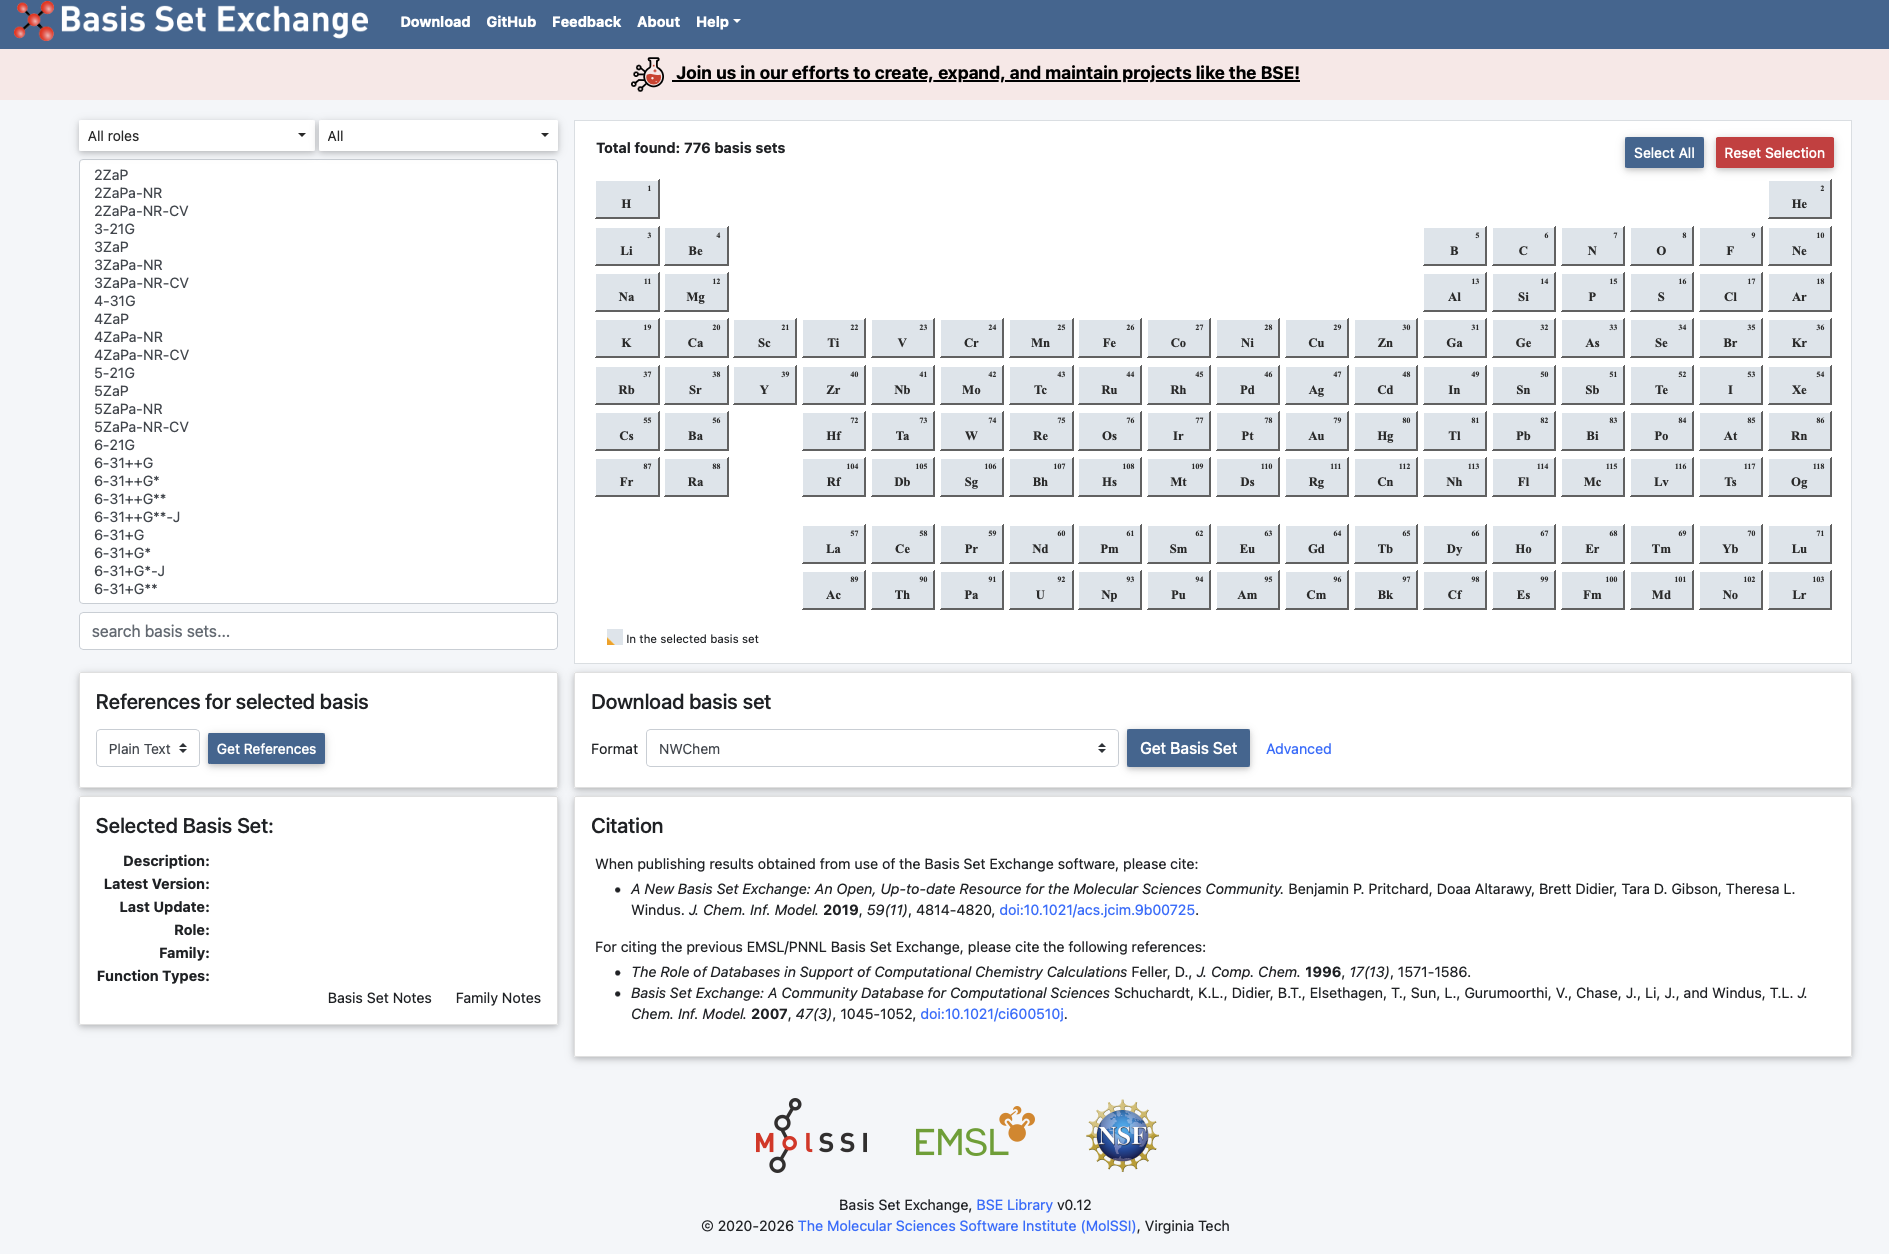
\includegraphics[width=0.72\textwidth]{BSE}
  \caption{The Basis Set Exchange provides standardized definitions for a
  large number of orbital and auxiliary basis sets \citep{Pritchard2019}.}
\end{figure}

\subsubsection{STO-$n$G minimal basis sets}

In an STO-$n$G basis, there is one contracted basis function for every occupied
orbital in the minimal atomic description. Each contracted GTO contains $n$
primitive GTOs, whose contraction coefficients and exponents are selected so
that the contraction approximates an STO. STO-$n$G bases are therefore minimal,
single-$\zeta$ basis sets; STO-3G is the most familiar member
\citep{Hehre1969}.
For hydrogen, Table~\ref{tab:hydrogen-sto3g} lists the three primitives in
the contraction, and Fig.~\ref{fig:hydrogen-sto3g} shows how their sum
approximates the Slater-type $1s$ orbital.
\begin{table}[htbp]
  \centering
  {\renewcommand{\arraystretch}{1.22}
  % Exact transcription of the hydrogen STO-3G shell in fig/STO-3G.png.
% Cross-checked against the Basis Set Exchange STO-3G hydrogen definition.
\begin{tabular}{crr}
\toprule
Primitive $i$ & Exponent $\alpha_i$ ($a_0^{-2}$) & Coefficient $D_i$\\
\midrule
1 & $3.425250914$ & $0.1543289673$\\
2 & $0.6239137298$ & $0.5353281423$\\
3 & $0.1688554040$ & $0.4446345422$\\
\bottomrule
\end{tabular}
}
  \caption{Primitive exponents and contraction coefficients for the hydrogen
  $1s$ function in STO-3G, with shell scale $1.00$. The dimensionless
  coefficients $D_i$ multiply normalized primitive Gaussians; $a_0$ is the
  Bohr radius. Values are transcribed without rounding from the Basis Set
  Exchange excerpt in the lecture slides and checked against its STO-3G
  hydrogen definition \citep{Hehre1969,Pritchard2019}.}
  \label{tab:hydrogen-sto3g}
\end{table}
\begin{figure}[htbp]
  \centering
  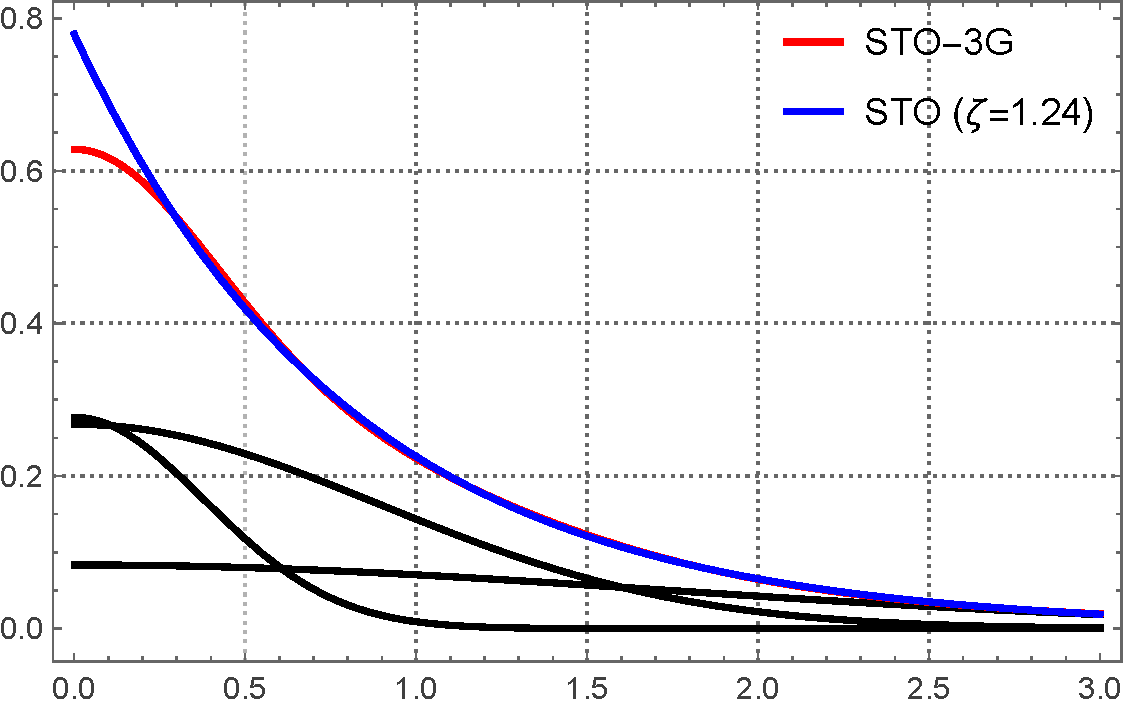
\includegraphics[width=0.80\textwidth]{STO}
  \caption{Radial dependence of the hydrogen $1s$ STO with
  $\zeta=1.24\,a_0^{-1}$ (blue) and its STO-3G approximation (red).
  The black curves are the three coefficient-weighted normalized Gaussian
  primitives whose sum forms the contraction, using the parameters in
  Table~\ref{tab:hydrogen-sto3g}. The horizontal coordinate is the distance
  $r$ from the nucleus in Bohr radii; the curves show spatial-orbital
  amplitudes, not radial probability densities. The plot is retained from
  the original lecture material.}
  \label{fig:hydrogen-sto3g}
\end{figure}

The quality of the contraction is controlled by $n$, but the molecular
orbital space still contains only the minimal number of functions. Such a
basis is useful for illustrating the construction, while its lack of extra
radial and angular flexibility limits quantitative accuracy.

\subsubsection{Pople split-valence basis sets}

Pople basis sets \citep{Hehre1972} extend the minimal description by splitting the valence space
and by adding optional diffuse and polarization shells. Their notation
explicitly records the contractions and augmentations. In
6-31+G*, the core function is contracted from six primitives; the valence
space is double-$\zeta$, with contractions of three and one primitives; the
``+'' adds diffuse functions to non-hydrogen atoms \citep{Clark1983}; and ``*'' adds polarization
functions to non-hydrogen atoms, conventionally a $d$ shell. In 6-311++G**,
the valence space is triple-$\zeta$ with contractions $3,1,1$ \citep{Krishnan1980}; the second
``+'' adds diffuse functions to hydrogen; and the second ``*'' adds
polarization functions to hydrogen. Finally, 6-311G(2df,2pd) adds two $d$ and
one $f$ polarization shells to non-hydrogen atoms, and two $p$ and one $d$
shell to hydrogen \citep{Frisch1984}.

The notation describes how the basis is assembled: the contraction pattern is
followed by symbols or parentheses identifying diffuse and polarization
functions. It is therefore more detailed than a simple label of basis size.

\subsubsection{Dunning correlation-consistent basis sets}

The correlation-consistent construction \citep{Dunning1989} organizes functions into successive
balanced layers designed to recover angular correlation systematically. The
main sequence is
\begin{equation}
  \text{cc-pVXZ},\qquad X=\mathrm{D,T,Q,5,6}
\end{equation}
In the basis names, D, T, and Q denote double-, triple-, and quadruple-$\zeta$
quality. The numerical cardinal number $X$ takes the corresponding values
$2,3,4,5,6$. A standard correlation-energy extrapolation
\citep{Helgaker1997} is
\begin{equation}
  \Ec(X)\approx\Ec^\text{CBS}+AX^{-3}
\end{equation}
Here $\Ec^\text{CBS}$ is the complete-basis-set correlation energy and $A$
is an extrapolation coefficient, not an atomic-center label.
Diffuse augmentation gives aug-cc-pVXZ, d-aug-cc-pVXZ, and t-aug-cc-pVXZ
\citep{Kendall1992}.
Core correlation is described by cc-pCVXZ, optimized for core--core and
core--valence correlation \citep{Woon1995}, or by cc-pwCVXZ, which weights the core--valence
contribution \citep{Peterson2002}.

The cardinal number $X$ labels the level of this hierarchy. Increasing $X$
adds both radial flexibility and a new layer of higher angular momentum, as
the explicit shell patterns below demonstrate.

For a second-row atom, the valence correlation-consistent sequence is
\begin{center}
\begin{tabular}{c@{\qquad}c}
\toprule
Basis & shell content\\
\midrule
cc-pVDZ & $3s2p1d$\\
cc-pVTZ & $4s3p2d1f$\\
cc-pVQZ & $5s4p3d2f1g$\\
aug-cc-pVDZ & $4s3p2d$\\
aug-cc-pVTZ & $5s4p3d2f$\\
aug-cc-pVQZ & $6s5p4d3f2g$\\
d-aug-cc-pVDZ & $5s4p3d$\\
d-aug-cc-pVTZ & $6s5p4d3f$\\
d-aug-cc-pVQZ & $7s6p5d4f3g$\\
\bottomrule
\end{tabular}
\end{center}
The successive entries make the layered construction explicit. For the
core--valence sequence, the corresponding decomposition is
\begin{align}
 \text{cc-pVDZ: }&3s2p1d=1s+2s2p1d\\
 \text{cc-pVTZ: }&4s3p2d1f=1s+3s3p2d1f\\
 \text{cc-pVQZ: }&5s4p3d2f1g=1s+4s4p3d2f1g\\
 \text{cc-pCVDZ: }&4s3p1d=2s1p+2s2p1d\\
 \text{cc-pCVTZ: }&6s5p3d1f=3s2p1d+3s3p2d1f\\
 \text{cc-pCVQZ: }&8s7p5d3f1g=4s3p2d1f+4s4p3d2f1g
\end{align}

\subsubsection{Jensen polarization-consistent basis sets}

Jensen's polarization-consistent sets \citep{Jensen2001} apply systematic improvement to HF and
Kohn--Sham calculations, with functions selected according to their energetic
importance. The sequence has shell contents
\begin{equation}
  \text{pc-0}:3s2p\quad
  \text{pc-1}:3s2p1d\quad
  \text{pc-2}:4s3p2d1f\quad
  \text{pc-3}:6s5p4d2f1g
\end{equation}
Thus pc-0 is unpolarized, pc-1 adds one polarization layer, and the later
members add systematically more radial and angular flexibility. Diffuse variants
are denoted aug-pc-$n$. Their HF convergence is described by the
extrapolation form \citep{Jensen2005}
\begin{equation}
  E_\text{HF}(L)=E_\text{HF}^\text{CBS}
  +A(L+1)\exp(-B\sqrt L)
\end{equation}
Here $L$ is the highest angular momentum present in the basis, while $A$ and
$B$ are extrapolation coefficients. This HF extrapolation is distinct from
the inverse-cubic correlation-energy extrapolation above.

These hierarchies illustrate why Gaussian bases are widely used: they are
compact, atom centered, chemically transferable, supported
by analytic integral technology, and available in systematic hierarchies.
They make all-electron calculations practical for light and medium elements,
and their locality supports integral screening and sparse algorithms. The
physical picture is that a molecule is assembled from atoms whose electron
distributions are distorted by their environment. Because the basis functions
move with the nuclei, nuclear derivatives contain Pulay terms in addition to
the derivatives of the electronic Hamiltonian.
Their principal limitations are the absent nuclear cusp, the incorrect
long-range Gaussian decay, basis-set superposition error, and possible linear
dependence when many diffuse functions are used. There is consequently no
single best Gaussian basis: the appropriate choice depends on the property,
the electronic-structure method, and the desired accuracy.

\subsubsection{Basis-set superposition error and counterpoise correction}

The locality that makes atom-centered bases compact also creates a possible
imbalance when fragment energies are compared. Atom-centered basis functions
belong formally to the complete calculation
rather than to immutable fragments. When two fragments approach one another,
each gains access to functions centered on the other, and the dimer and
isolated-fragment energies no longer possess equivalent variational
flexibility.

Let $E_X^Y$ denote the energy of system $X$ evaluated in basis $Y$. In a
dimer $AB$, each fragment can borrow the basis functions of the other fragment
as ghost functions. The variational principle therefore gives
\begin{equation}
  E_A^{AB}\leq E_A^A\qquad E_B^{AB}\leq E_B^B
\end{equation}
which makes the uncorrected interaction energy
\begin{equation}
  \Delta E_\text{int}=E_{AB}^{AB}-E_A^A-E_B^B
\end{equation}
artificially too attractive. The Boys--Bernardi counterpoise correction
\citep{BoysBernardi1970} uses
the full dimer basis for every term,
\begin{equation}
  \Delta E_\text{int}^\text{CP}
  =E_{AB}^{AB}-E_A^{AB}-E_B^{AB}
\end{equation}
and the basis-set superposition error (BSSE) is
\begin{equation}
  \mathrm{BSSE}
  =\Delta E_\text{int}^\text{CP}-\Delta E_\text{int}
  =(E_A^A-E_A^{AB})+(E_B^B-E_B^{AB})\geq0
\end{equation}

The partner's basis functions are retained as ghost functions: they provide
variational flexibility but carry neither electrons nor nuclear charge. The
counterpoise expression thereby compares the dimer and both fragments in the
same one-electron space.

\begin{figure}[htbp]
 \centering
 \begin{tikzpicture}[
  atom/.style={circle,draw,minimum size=0.7cm,inner sep=0pt},
  ghost/.style={circle,draw,dashed,minimum size=0.7cm,inner sep=0pt},
  basis/.style={ellipse,draw,minimum width=1.5cm,minimum height=1.0cm},
  ghostbasis/.style={ellipse,draw,dashed,minimum width=1.5cm,minimum height=1.0cm}]
  \node at (-4.5,1.6) {$E_{\red A}^{\blue A}$};
  \node[basis] at (-4.5,0) {};
  \node[atom] at (-4.5,0) {$A$};
  \node at (-4.5,-0.9) {\small basis on $A$ only};
  \node at (0,1.6) {$E_{\red A}^{\blue{AB}}$};
  \node[basis] at (-0.9,0) {};
  \node[atom] at (-0.9,0) {$A$};
  \node[ghostbasis,hfViolet] at (0.9,0) {};
  \node[ghost,hfViolet] at (0.9,0) {$B$};
  \node at (0,-0.9) {\small basis on $A$ + \violet{ghost basis} on $B$};
  \node at (4.9,1.6) {$E_{\red{AB}}^{\blue{AB}}$};
  \node[basis] at (4.0,0) {};
  \node[atom] at (4.0,0) {$A$};
  \node[basis] at (5.8,0) {};
  \node[atom] at (5.8,0) {$B$};
  \node at (4.9,-0.9) {\small full dimer basis};
 \end{tikzpicture}
 \caption{A fragment in its own basis, the same fragment supplemented by
 ghost functions, and the full dimer. Dashed violet shapes retain basis
 functions without adding nuclear charge or electrons.}
 \label{fig:ghost-basis}
\end{figure}

\subsection{Effective core potentials and pseudopotentials}

Core electrons are numerous and spatially compact, yet they often participate
only indirectly in chemical bonding. Effective core potentials (ECPs)
exploit this
separation by replacing selected core electrons and their nuclear interaction
with an operator acting on the remaining explicit electrons.

The key idea of an effective core potential \citep{WadtHay1985} is to treat only the chemically
relevant electrons explicitly. It replaces the nuclear attraction and the
chemically inactive core electrons by an effective one-electron operator,
\begin{equation}
 \hh(\br)=-\frac{\nabla^2}{2}
 -\sum_A\frac{Z_A}{\abs{\br-\bR_A}}
 \longrightarrow
 \hh^\text{ECP}(\br)=-\frac{\nabla^2}{2}
 -\sum_A\frac{\green{Q_A}}{\abs{\br-\bR_A}}
 +\sum_A\hat U_A^\text{ECP}(\br)
 \qquad \green{Q_A}=Z_A-N_A^\text{core}
\end{equation}
Here $N_A^\text{core}$ is the number of electrons removed by the ECP on atom
$A$, and $Q_A$ is the charge of the remaining ionic core. It is not the
population-analysis charge $q_A$ introduced earlier.
This lowers the cost by reducing the number of explicit electrons and removing
the basis functions needed for core orbitals. It can incorporate
scalar-relativistic effects and, with a suitable operator, spin--orbit
coupling, and it can be used in both molecular and periodic calculations with
Gaussian or plane-wave bases. The price is a new class of one-electron
integrals that can be difficult to evaluate; core properties are not described
explicitly, and the accuracy depends on the ECP quality.

For one center, with $r$ measured from that center and $L$ labeling the local
channel, a common semilocal form is
\begin{equation}
  U^\text{ECP}=U_L(r)+
  \sum_{\ell=0}^{L-1}\sum_{m=-\ell}^{\ell}
  \ket{Y_{\ell m}}U_\ell(r)\bra{Y_{\ell m}}
\end{equation}
The first term is local, or unprojected; the remaining angular-momentum
channels are nonlocal, or projected. Their radial parts are generally expanded
as
\begin{equation}
  U_\ell(r)=\sum_kD_{\ell k}r^{n_{\ell k}}
  \exp(-\eta_{\ell k}r^2)
  \qquad n_{\ell k}\in\{-2,-1,0\}
\end{equation}
The $D_{\ell k}$ and $\eta_{\ell k}$ are fitted parameters. Although these are
one-electron operators, their angular projectors make the integrals nontrivial.

For silver, a large-core ECP removes 36 electrons and treats explicitly the
$4d^{10}5s^1$ shells, leaving 11 electrons. A small-core ECP removes 28
electrons and retains $4s^24p^64d^{10}5s^1$, leaving 19 explicit electrons;
the semicore $4s$ and $4p$ shells are therefore retained, providing more
flexibility at higher cost. Several Gaussian-basis ECP families are commonly
used. LANL \citep{WadtHay1985} and SBK/SBKJC \citep{Stevens1992} are established families; in particular, LANL2DZ
combines an ECP with a double-$\zeta$ valence basis. The
\href{https://www.tc.uni-koeln.de/PP/clickpse.en.html}
{Stuttgart/Cologne energy-consistent pseudopotentials} are offered with
different core sizes and dedicated bases \citep{Bergner1993}, while the def2-ECPs are paired with
the def2 bases of Weigend and Ahlrichs \citep{WeigendAhlrichs2005}. The Burkatzki--Filippi--Dolg (BFD)
potentials were developed for quantum Monte Carlo calculations \citep{Burkatzki2007}, whereas the
\href{https://pseudopotentiallibrary.org}{correlation-consistent ECPs
(ccECPs)} were developed for high-accuracy correlated many-body methods \citep{Bennett2017}.
Most ECPs have dedicated basis sets.

The core size is consequently a controlled compromise. A large-core potential
is cheaper, whereas a small-core potential retains more semicore response and
flexibility. Consistency requires the ECP and its accompanying valence basis
to be treated as a matched pair.

\section{Molecular integrals over Gaussian functions}
\label{sec:gaussian-integrals}

Once the orbital basis and any effective core potential have been selected,
the abstract matrix elements of the finite-basis Hartree--Fock equations must
be evaluated. Gaussian functions are especially valuable because their
products and derivatives can be reduced to a small set of fundamental
integrals. The discussion below develops that reduction from overlap and
one-electron terms to four-center electron-repulsion integrals, and then shows
how recurrence relations and screening turn the resulting formulas into a
practical algorithm \citep{Gill1994}.

\subsection{The Gaussian product theorem and overlap integrals}
\label{sec:gaussian-product}

The efficiency of Gaussian basis sets follows from a closure property that
reduces multicenter products to single-center quantities. The central
algebraic fact behind Gaussian integral technology is the
Gaussian product rule: the product of two Gaussians is another Gaussian.
This closure property underlies the classical Gaussian integral formulation
of Boys \citep{Boys1950}.
Writing the $s$-type Gaussian factors as
\begin{equation}
 G_{\red{\alpha},\red{\bA}}(\br)
 =\exp[-\red{\alpha}\abs{\br-\red{\bA}}^2]
 \qquad
 G_{\blue{\beta},\blue{\bB}}(\br)
 =\exp[-\blue{\beta}\abs{\br-\blue{\bB}}^2]
\end{equation}
then
\begin{equation}
 G_{\red{\alpha},\red{\bA}}(\br)
 G_{\blue{\beta},\blue{\bB}}(\br)
 =K_{\violet{\zeta},\violet{\bP}}
 G_{\violet{\zeta},\violet{\bP}}(\br)
 \label{eq:gaussian-product}
\end{equation}
with
\begin{equation}
 \violet{\zeta}=\red{\alpha}+\blue{\beta}
 \qquad
 \violet{\bP}=\frac{\red{\alpha\bA}+\blue{\beta\bB}}
 {\red{\alpha}+\blue{\beta}}
\end{equation}
and
\begin{equation}
 K_{\violet{\zeta},\violet{\bP}}
 =\exp[-\frac{\red{\alpha}\blue{\beta}}
 {\red{\alpha}+\blue{\beta}}\abs{\red{\bA}-\blue{\bB}}^2]
\end{equation}
The product center $\bP$ lies on the line joining $\bA$ and $\bB$ and is
weighted toward the Gaussian with the larger exponent. The prefactor contains
the dependence on the separation of the original centers: its Gaussian decay
makes distant pairs rapidly negligible. The bold $\bP$ here denotes a
coordinate, not the density matrix used in the HF equations.

For two $s$ Gaussians, the overlap illustrates Cartesian factorization:
\begin{align}
 \int G_{\red{\alpha},\red{\bA}}(\br)
 G_{\blue{\beta},\blue{\bB}}(\br)\dd\br
 &=K_{\violet{\zeta},\violet{\bP}}
   \int G_{\violet{\zeta},\violet{\bP}}(\br)\dd\br\\
 &=K_{\violet{\zeta},\violet{\bP}}
 \qty(\int_{-\infty}^{+\infty}e^{-\violet{\zeta}x^2}\dd x)
 \qty(\int_{-\infty}^{+\infty}e^{-\violet{\zeta}y^2}\dd y)
 \qty(\int_{-\infty}^{+\infty}e^{-\violet{\zeta}z^2}\dd z)\\
 &=K_{\violet{\zeta},\violet{\bP}}
 \qty(\frac{\pi}{\violet{\zeta}})^{3/2}
\end{align}

\subsection{One-electron Gaussian integrals}

Once the product theorem has combined two basis functions, overlap, kinetic,
and nuclear-attraction integrals reduce to Gaussian moments about the product
center. The $s$-type formulas expose the essential structure before angular
momentum is introduced.

\paragraph{Kinetic-energy integral.}

The Laplacian of an $s$ Gaussian is
\begin{equation}
 -\frac12\laplacian G_{\blue{\beta},\blue{\bB}}(\br)
 =\qty[3\blue{\beta}-2\blue{\beta}^2
 \abs{\br-\blue{\bB}}^2]G_{\blue{\beta},\blue{\bB}}(\br)
\end{equation}
Consequently, using the Gaussian product theorem
\eqref{eq:gaussian-product}, its kinetic-energy integral becomes
\begin{align}
 -\frac12\int G_{\red{\alpha},\red{\bA}}(\br)\laplacian
 G_{\blue{\beta},\blue{\bB}}(\br)\dd\br
 &=\int G_{\red{\alpha},\red{\bA}}(\br)
 \qty[3\blue{\beta}-2\blue{\beta}^2
 \abs{\br-\blue{\bB}}^2]
 G_{\blue{\beta},\blue{\bB}}(\br)\dd\br\\
 &=\frac{\red{\alpha}\blue{\beta}}{\violet{\zeta}}
 \qty[3-2\frac{\red{\alpha}\blue{\beta}}{\violet{\zeta}}
 \abs{\red{\bA}-\blue{\bB}}^2]
 K_{\violet{\zeta},\violet{\bP}}
 \qty(\frac{\pi}{\violet{\zeta}})^{3/2}
\end{align}

The result has the same overlap prefactor as the preceding integral. The
additional polynomial factor is the consequence of differentiating the
Gaussian centered at $\blue{\bB}$ twice. It contains both a local curvature
term, $3\blue{\beta}$, and a term that depends on the separation of the two
centers.

\paragraph{Nuclear-attraction integral.}

For a nucleus of charge $Z_C$ located at $\bC$, the nuclear-attraction
integral introduces the function $F_0$, the zeroth-order Boys function defined
in Eq.~\eqref{eq:boys-functions}:
\begin{align}
 -Z_C\int G_{\red{\alpha},\red{\bA}}(\br)
 \frac{1}{\abs{\br-\bC}}
 G_{\blue{\beta},\blue{\bB}}(\br)\dd\br
 &=-Z_CK_{\violet{\zeta},\violet{\bP}}
 \int\frac{e^{-\violet{\zeta}\abs{\br-\violet{\bP}}^2}}
 {\abs{\br-\bC}}\dd\br\\
 &=-\frac{2Z_C}{\sqrt\pi}K_{\violet{\zeta},\violet{\bP}}
 \int_0^\infty\dd t\int
 e^{-\violet{\zeta}\abs{\br-\violet{\bP}}^2}
 e^{-t^2\abs{\br-\bC}^2}\dd\br\\
 &=-\frac{2\pi Z_C}{\violet{\zeta}}
 K_{\violet{\zeta},\violet{\bP}}
 F_0\qty(\violet{\zeta}\abs{\violet{\bP}-\bC}^2)
\end{align}

\subsection{Four-center electron-repulsion integrals}

Electron-repulsion integrals are the most numerous quantities in conventional
molecular Hartree--Fock theory. Four basis functions and the nonseparable
Coulomb kernel appear, but the product theorem reduces the four original
centers to two Gaussian product centers.

\paragraph{Gaussian-pair reduction.}

Applying the Gaussian product rule to the $s$-type factors on both electron
coordinates gives
\begin{align}
 \rbraket{\red{\ba}\blue{\bb}}{\orange{\bc}\green{\bd}}
 &=\iint G_{\red{\alpha},\red{\bA}}(\br_1)
 G_{\blue{\beta},\blue{\bB}}(\br_1)\frac{1}{r_{12}}
 G_{\orange{\gamma},\orange{\bC}}(\br_2)
 G_{\green{\delta},\green{\bD}}(\br_2)\dd\br_1\dd\br_2\\
 &=K_{\violet{\zeta},\violet{\bP}}
 K_{\purple{\eta},\purple{\bQ}}
 \iint G_{\violet{\zeta},\violet{\bP}}(\br_1)
 \frac{1}{r_{12}}G_{\purple{\eta},\purple{\bQ}}(\br_2)
 \dd\br_1\dd\br_2
\end{align}
The second pair has combined exponent $\eta=\gamma+\delta$ and product
center $\bQ=(\gamma\bC+\delta\bD)/\eta$, with a prefactor
$K_{\eta,\bQ}$ defined in the same way as for the first pair.
There are formally $\order{K^4}$ ERIs, although only $\order{K^2}$ are
significant in a sufficiently large, spatially extended system.

\paragraph{Functions, shell pairs, and shell quartets.}

The notation distinguishes individual functions from shells and primitives
from contractions. Thus $\sbra{\red{\ba}\blue{\bb}}$ is one primitive bra,
whereas $\sbra{\red a\blue b}$ is a complete primitive shell pair;
$\sbraket{\red{\ba}\blue{\bb}}{\orange{\bc}\green{\bd}}$ is one primitive
integral, whereas $\sbraket{\red a\blue b}{\orange c\green d}$ is a primitive
shell quartet. Likewise, $\rbra{\red{\ba}\blue{\bb}}$ and
$\rbra{\red a\blue b}$ denote a contracted bra and contracted shell pair,
and $\rbraket{\red{\ba}\blue{\bb}}{\orange{\bc}\green{\bd}}$ and
$\rbraket{\red a\blue b}{\orange c\green d}$ denote a contracted integral
and a contracted shell quartet.

\subsubsection{The fundamental $ssss$ integral}

Higher-angular-momentum ERIs can be generated from a hierarchy of fundamental
$s$-type quantities. The derivation begins by replacing the Coulomb operator
with its Laplace representation, after which every Cartesian coordinate enters
through an ordinary Gaussian integral.

For four primitive $s$ functions,
\begin{align}
 \sbraket{\bs\bs}{\bs\bs}
 &=K_{\violet{\zeta},\violet{\bP}}
 K_{\purple{\eta},\purple{\bQ}}
 \iint G_{\violet{\zeta},\violet{\bP}}(\br_1)
 \frac{1}{r_{12}}G_{\purple{\eta},\purple{\bQ}}(\br_2)
 \dd\br_1\dd\br_2\\
 &=K_{\violet{\zeta},\violet{\bP}}
 K_{\purple{\eta},\purple{\bQ}}
 \iint e^{-\violet{\zeta}\abs{\br_1-\violet{\bP}}^2}
 \frac{1}{r_{12}}
 e^{-\purple{\eta}\abs{\br_2-\purple{\bQ}}^2}
 \dd\br_1\dd\br_2
\end{align}
The Laplace transform
\begin{equation}
 \frac{1}{r_{12}}=\frac{2}{\sqrt\pi}\int_0^\infty
 e^{-t^2r_{12}^2}\dd t
 =\frac{2}{\sqrt\pi}\int_0^\infty
 e^{-t^2(x_1-x_2)^2}e^{-t^2(y_1-y_2)^2}
 e^{-t^2(z_1-z_2)^2}\dd t
\end{equation}
turns the six-dimensional integral into three Cartesian factors:
\begin{align}
 \sbraket{\bs\bs}{\bs\bs}
 ={}&\frac{2}{\sqrt\pi}K_{\violet{\zeta},\violet{\bP}}
 K_{\purple{\eta},\purple{\bQ}}\int_0^\infty\dd t
 \qty[\iint e^{-\violet{\zeta}(x_1-\violet P_x)^2}
 e^{-t^2(x_1-x_2)^2}e^{-\purple{\eta}(x_2-\purple Q_x)^2}
 \dd x_1\dd x_2]\\
 &\cdot\qty[\iint e^{-\violet{\zeta}(y_1-\violet P_y)^2}
 e^{-t^2(y_1-y_2)^2}e^{-\purple{\eta}(y_2-\purple Q_y)^2}
 \dd y_1\dd y_2]\\
 &\cdot\qty[\iint e^{-\violet{\zeta}(z_1-\violet P_z)^2}
 e^{-t^2(z_1-z_2)^2}e^{-\purple{\eta}(z_2-\purple Q_z)^2}
 \dd z_1\dd z_2]
\end{align}

Defining
\begin{equation}
 \vartheta=\frac{\violet{\zeta}\purple{\eta}}
 {\violet{\zeta}+\purple{\eta}}
\end{equation}
the Cartesian integrations yield, step by step,
\begin{align}
 \sbraket{\bs\bs}{\bs\bs}
 ={}&\frac{2}{\sqrt\pi}K_{\violet{\zeta},\violet{\bP}}
 K_{\purple{\eta},\purple{\bQ}}\int_0^\infty
 \prod_{i=x,y,z}\qty[
 \frac{\pi}{\sqrt{\violet{\zeta}\purple{\eta}}}
 \frac{\exp[-\vartheta(\violet P_i-\purple Q_i)^2
 t^2/(t^2+\vartheta)]}
 {\sqrt{1+t^2/\vartheta}}]\dd t\\
 ={}&\frac{2\pi^{5/2}}
 {(\violet{\zeta}\purple{\eta})^{3/2}}
 K_{\violet{\zeta},\violet{\bP}}K_{\purple{\eta},\purple{\bQ}}
 \int_0^\infty
 \frac{\exp[-\vartheta\abs{\violet{\bP}-\purple{\bQ}}^2
 t^2/(t^2+\vartheta)]}{(1+t^2/\vartheta)^{3/2}}\dd t
\end{align}
With the substitution $t^2=\vartheta u^2/(1-u^2)$,
\begin{align}
 \sbraket{\bs\bs}{\bs\bs}
 ={}&\sqrt{\frac{4\vartheta}{\pi}}
 \qty(\frac{\pi}{\violet{\zeta}})^{3/2}
 K_{\violet{\zeta},\violet{\bP}}
 \qty(\frac{\pi}{\purple{\eta}})^{3/2}
 K_{\purple{\eta},\purple{\bQ}}
 \underbrace{\int_0^1e^{-\vartheta
 \abs{\violet{\bP}-\purple{\bQ}}^2u^2}\dd u}
 _{F_0(\vartheta\abs{\violet{\bP}-\purple{\bQ}}^2)}
\end{align}
The zero angular-momentum vector $\bO=(0,0,0)$ denotes an $s$ function in
this integral notation. The fundamental auxiliary notation is therefore
\begin{equation}
 \sbraket{\bO\bO}{\bO\bO}^{(0)}
 =\sqrt{\frac{4\vartheta}{\pi}}
 \qty(\frac{\pi}{\violet{\zeta}})^{3/2}K_{\violet{\zeta},\violet{\bP}}
 \qty(\frac{\pi}{\purple{\eta}})^{3/2}K_{\purple{\eta},\purple{\bQ}}
 F_0\qty(\vartheta\abs{\violet{\bP}-\purple{\bQ}}^2)
\end{equation}

The original six-dimensional Coulomb integral has thus been reduced to
elementary Gaussian prefactors and a one-dimensional function. This reduction
is the foundation of the recurrence construction below.

\subsubsection{Boys functions and auxiliary integrals}
\label{sec:boys-functions}

The remaining one-dimensional integral is collected into the generalized Boys
function. Here $m$ is a nonnegative integer order and $x$ a nonnegative,
dimensionless argument, not a Cartesian coordinate:
\begin{equation}
 F_m(x)=\int_0^1t^{2m}\exp(-xt^2)\dd t
 \qquad
 F_0(x)=\sqrt{\frac{\pi}{4x}}\erf(\sqrt x)
 \label{eq:boys-functions}
\end{equation}
At the origin, the exponential becomes unity and the limiting value follows
directly:
\begin{equation}
 F_m(0)=\int_0^1t^{2m}\dd t=\frac{1}{2m+1}
\end{equation}
This limit is particularly useful because the expression for $F_0(x)$ in
terms of the error function has an apparent singularity at $x=0$, although
the Boys function itself is perfectly finite there.

In implementations, $F_m(x)$ is evaluated from pretabulated grid values and
a Taylor expansion, often with a Chebyshev interpolation table \citep{Gill1994}. Lower orders
are then obtained by the downward recurrence
\begin{equation}
 F_m(x)=\frac{2xF_{m+1}(x)+\exp(-x)}{2m+1}
\end{equation}
This downward recurrence is numerically stable, whereas upward recursion can
become unstable for small $x$. At large $x$,
\begin{equation}
 F_m(x)\sim\frac{(2m-1)!!}{2^{m+1}}
 \sqrt{\frac{\pi}{x^{2m+1}}}
\end{equation}

The physical $ssss$ integral contains only $F_0$, but differentiation to
generate angular momentum produces higher Boys orders. It is therefore useful
to define the complete hierarchy
\begin{equation}
 \sbraket{\bO\bO}{\bO\bO}^{(\red m)}
 =\sqrt{\frac{4\vartheta}{\pi}}
 \qty(\frac{\pi}{\violet{\zeta}})^{3/2}K_{\violet{\zeta},\violet{\bP}}
 \qty(\frac{\pi}{\purple{\eta}})^{3/2}K_{\purple{\eta},\purple{\bQ}}
 F_{\red m}\qty(\vartheta\abs{\violet{\bP}-\purple{\bQ}}^2)
\end{equation}
The $m=0$ member is the physical $ssss$ ERI; the $m>0$ members are auxiliary
intermediates. Angular-momentum recurrences couple orders $m$ and $m+1$.
For total angular momentum $L=a+b+c+d$, fundamental auxiliary integrals are
needed through $m=L$.

The recurrence construction must therefore retain the necessary Boys orders
alongside the angular-momentum labels.

\subsubsection{Obara--Saika recurrence relations}
\label{sec:os-recurrences}

Deriving a separate closed expression for every angular-momentum combination
would be inefficient. Obara--Saika instead uses differentiation identities to
generate the required quantities recursively from lower-angular-momentum
integrals \citep{ObaraSaika1986}.

\paragraph{Generating angular momentum vertically.}

Here $i$ labels a Cartesian direction, $x$, $y$, or $z$, rather than an
occupied orbital. The vector $\bI_i$ has unit component in direction $i$ and
zero components in the other two directions. For an unnormalized primitive
Cartesian Gaussian, the key identity is
\begin{equation}
 \pdv{\sket{\red{\ba}}}{A_i}
 =2\alpha\sket{\red{\ba}+\bI_i}
 -a_i\sket{\red{\ba}-\bI_i}
 \qquad
 \sket{\red{\ba}+\bI_i}
 =\frac{1}{2\alpha}\qty[
 \pdv{\sket{\red{\ba}}}{A_i}
 +a_i\sket{\red{\ba}-\bI_i}]
\end{equation}
Applying this identity to auxiliary ERIs creates the Obara--Saika vertical
recurrence relations (VRRs), so that integrals are built recursively rather
than independently:
\begin{equation}
 \sbraket{00}{00}^{(m)}\longrightarrow
 \sbraket{\red a0}{00}^{(m)}\longrightarrow
 \sbraket{\red a0}{\orange c0}^{(m)}
\end{equation}

On the bra pair, angular momentum is built on $\bA$ according to
\begin{align}
 \sbraket{(\red{\ba}+\bI_i)\bO}{\bO\bO}^{(m)}
 ={}&(P_i-A_i)\sbraket{\red{\ba}\bO}{\bO\bO}^{(m)}
 -\frac{\eta}{\zeta+\eta}(P_i-Q_i)
 \sbraket{\red{\ba}\bO}{\bO\bO}^{(m+1)}\notag\\
 &+\frac{a_i}{2\zeta}\qty[
 \sbraket{(\red{\ba}-\bI_i)\bO}{\bO\bO}^{(m)}
 -\frac{\eta}{\zeta+\eta}
 \sbraket{(\red{\ba}-\bI_i)\bO}{\bO\bO}^{(m+1)}]
\end{align}
On the ket pair, angular momentum is built on $\bC$ according to
\begin{align}
 \sbraket{\red{\ba}\bO}{(\orange{\bc}+\bI_i)\bO}^{(m)}
 ={}&(Q_i-C_i)\sbraket{\red{\ba}\bO}{\orange{\bc}\bO}^{(m)}
 -\frac{\zeta}{\zeta+\eta}(Q_i-P_i)
 \sbraket{\red{\ba}\bO}{\orange{\bc}\bO}^{(m+1)}\notag\\
 &+\frac{c_i}{2\eta}\qty[
 \sbraket{\red{\ba}\bO}{(\orange{\bc}-\bI_i)\bO}^{(m)}
 -\frac{\zeta}{\zeta+\eta}
 \sbraket{\red{\ba}\bO}{(\orange{\bc}-\bI_i)\bO}^{(m+1)}]\notag\\
 &+\frac{a_i}{2(\zeta+\eta)}
 \sbraket{(\red{\ba}-\bI_i)\bO}{\orange{\bc}\bO}^{(m+1)}
\end{align}

The signs of the product-center terms can be checked directly from the
fundamental integral. With $T=\vartheta\abs{\bP-\bQ}^2$, the definition of
the Boys function gives $\dv{F_m(T)}{T}=-F_{m+1}(T)$. Since
$\pdv{P_i}{A_i}=\alpha/\zeta$, differentiating the fundamental integral
and dividing by $2\alpha$ yields
\begin{equation}
 \sbraket{\bI_i\bO}{\bO\bO}^{(m)}
 =(P_i-A_i)\sbraket{\bO\bO}{\bO\bO}^{(m)}
 -\frac{\vartheta}{\zeta}(P_i-Q_i)
 \sbraket{\bO\bO}{\bO\bO}^{(m+1)}
\end{equation}
Here $\vartheta/\zeta=\eta/(\zeta+\eta)$. The ket-pair result follows
by exchanging the two pairs. The derivative argument fixes both
product-center terms to have negative signs.

The required angular-momentum build and contraction are organized as
\begin{equation}
 \sbraket{00}{00}^{(m)}
 \xrightarrow{\red{\mathrm{VRR}}}
 \sbraket{\red a0}{\orange c0}^{(m)}
 \xrightarrow{\orange{\mathrm{contraction}}}
 \rbraket{\red a0}{\orange c0}
 \xrightarrow{\blue{\mathrm{HRR}}}
 \rbraket{\red a\blue b}{\orange c\green d}
\end{equation}
The VRRs create angular momentum on one center of each Gaussian pair;
contraction combines primitive integrals; and the horizontal recurrence
relations (HRRs) redistribute angular momentum within each pair.

\paragraph{Redistributing angular momentum horizontally.}

Once angular momentum has been generated on one center, it is shifted to the
other through
\begin{equation}
 \sbraket{\red{\ba}(\blue{\bb}+\bI_i)}
 {\orange{\bc}\green{\bd}}
 =\sbraket{(\red{\ba}+\bI_i)\blue{\bb}}
 {\orange{\bc}\green{\bd}}
 +(A_i-B_i)\sbraket{\red{\ba}\blue{\bb}}
 {\orange{\bc}\green{\bd}}
\end{equation}
An analogous relation transfers angular momentum from $\bC$ to $\bD$.
Because the HRR depends only on $A_i-B_i$, it is independent of the Gaussian
exponents and applies directly to contracted integrals:
\begin{equation}
 \rbraket{\red{\ba}(\blue{\bb}+\bI_i)}
 {\orange{\bc}\green{\bd}}
 =\rbraket{(\red{\ba}+\bI_i)\blue{\bb}}
 {\orange{\bc}\green{\bd}}
 +(A_i-B_i)\rbraket{\red{\ba}\blue{\bb}}
 {\orange{\bc}\green{\bd}}
\end{equation}

The late-contraction algorithm begins by
computing the required Boys functions $F_m(T)$ from
Section~\ref{sec:boys-functions} and forming the fundamental
auxiliary integrals $\sbraket{00}{00}^{(m)}$. The VRRs are then used to build
angular momentum on $\bA$ and $\bC$, after which the primitive integrals are
contracted. Finally, the exponent-independent HRRs transfer angular momentum
according to $\bA\rightarrow\bB$ and $\bC\rightarrow\bD$.
This combination of vertical and horizontal recurrences is the
Head--Gordon--Pople late-contraction strategy \citep{HeadGordonPople1988}; the vertical recurrences are
those of Obara--Saika. Thus the expensive exponent-dependent recurrences are performed before
contraction, whereas the cheap exponent-independent HRRs are performed after
contraction.

The resulting reduction in the number of quantities handled by the HRRs
complements the screening savings considered next.

\subsection{Integral bounds, screening, and direct SCF}
\label{sec:integral-screening}

A formal count of $K^4$ ERIs greatly overestimates the useful work for large
local systems because most products of distant basis functions are negligible.
Screening converts this locality into a computational saving by testing a
cheap upper bound before evaluating an integral or shell quartet.

\paragraph{Cauchy--Schwarz bounds.}

A useful ERI upper bound must be simple and inexpensive, strong enough to be a
good estimate, and scaling consistent, meaning
$N_\text{sig}=\order{N_\text{upper}}$. Here $N_\text{sig}$ counts significant
integrals and $N_\text{upper}$ counts those retained by the bound at the
chosen threshold. The Cauchy--Schwarz inequality gives
\begin{equation}
 \abs{\rbraket{\red{\ba}\blue{\bb}}{\orange{\bc}\green{\bd}}}
 \leq
 \sqrt{\rbraket{\red{\ba}\blue{\bb}}{\red{\ba}\blue{\bb}}}
 \sqrt{\rbraket{\orange{\bc}\green{\bd}}{\orange{\bc}\green{\bd}}}
\end{equation}
or, in terms of the Gaussian product centers,
\begin{equation}
 \abs{\rbraket{\violet{\bP}}{\purple{\bQ}}}
 \leq\sqrt{\rbraket{\violet{\bP}}{\violet{\bP}}}
 \sqrt{\rbraket{\purple{\bQ}}{\purple{\bQ}}}
\end{equation}
The integral $\rbraket{\violet{\bP}}{\purple{\bQ}}$ should decay as
$1/\abs{\violet{\bP}-\purple{\bQ}}$ or faster. The product on the right has
no information about the separation between the two charge distributions, so
the Cauchy--Schwarz bound is rigorous and cheap but not tight for well-separated
shell pairs. Even so, a cheap upper bound avoids evaluating negligible ERIs.
The practical use of integral bounds in direct-SCF screening is discussed by
\citet{HaserAhlrichs1989}.

\paragraph{Shell-quartet screening.}

At the individual-integral level, only $\order{K^2}$ diagonal factors
$\rbraket{\red{\ba}\blue{\bb}}{\red{\ba}\blue{\bb}}$ are required to bound
$\order{K^4}$ four-center integrals. More efficiently, define a shell-pair
bound
\begin{equation}
 Q_{\red a\blue b}
 =\max_{\substack{\red{\ba}\in a\\\blue{\bb}\in b}}
 \sqrt{\rbraket{\red{\ba}\blue{\bb}}{\red{\ba}\blue{\bb}}}
\end{equation}
Then an entire shell class obeys
\begin{equation}
 \abs{\rbraket{\red a\blue b}{\orange c\green d}}
 \leq Q_{\red a\blue b}Q_{\orange c\green d}
\end{equation}
For a positive screening threshold $\tau$, if
\begin{equation}
 Q_{\red a\blue b}Q_{\orange c\green d}<\tau
\end{equation}
the entire shell quartet can be discarded. This is consequential: even the
simple $\rbraket{dd}{dd}$ class contains 1296 Cartesian integrals.

The number of significant integrals may be represented by
\begin{equation}
 \rbraket{\red{\ba}\blue{\bb}}{\orange{\bc}\green{\bd}}
 \equiv\rmel{\red{\ba}\blue{\bb}}{\chO_2}
 {\orange{\bc}\green{\bd}}
 \qquad N_\text{sig}=cK^\alpha
\end{equation}
Here $K$ is the number of basis functions, $c$ is a proportionality factor,
and $\alpha$ is the effective scaling exponent. The count $N_\text{sig}$
is distinct from the electron number $N$ used in the HF derivations.
The numerical data in Table~\ref{tab:screening-scaling} contrast the long-range Coulomb operator with a
short-range Gaussian operator:
\begin{table}[htbp]
\centering
\small
\begin{tabular}{lrrrrr}
\toprule
& &\multicolumn{2}{c}{\red{$\chO=r_{12}^{-1}$}}
&\multicolumn{2}{c}{\orange{$\chO=e^{-r_{12}^2}$}}\\
\cmidrule(lr){3-4}\cmidrule(lr){5-6}
Molecule&$K$&$N_\text{sig}$&$\alpha$&$N_\text{sig}$&$\alpha$\\
\midrule
propene&12&1,625&---&1,650&---\\
butadiene&16&5,020&3.9&5,020&3.9\\
hexatriene&24&24,034&3.9&23,670&3.8\\
octatetraene&32&63,818&3.4&52,808&2.8\\
decapentaene&40&119,948&2.8&81,404&1.9\\
dodecahexaene&48&192,059&2.6&109,965&1.6\\
\bottomrule
\end{tabular}
\caption{Numbers of significant integrals and effective scaling exponents
for Coulomb and short-range Gaussian operators. Numerical data reproduced
from the lecture slides.}
\label{tab:screening-scaling}
\end{table}
The Coulomb interaction remains long ranged, so its effective exponent falls
more slowly than that of the short-range Gaussian operator. Nevertheless, the
data show that the number of numerically significant Coulomb integrals grows
much more slowly than the formal quartic count in sufficiently large systems.

The complete integral-evaluation strategy has three components. The target
quantities are the two-electron integrals
$\rbraket{\ba\bb}{\bc\bd}$. Their construction requires the fundamental
integrals $\rbraket{\bO\bO}{\bO\bO}^{(m)}$, the recurrence relations,
represented schematically by
$\rbraket{(\ba+\bI_i)\bO}{\bO\bO}
=\rbraket{\ba\bO}{\bO\bO}
+\rbraket{(\ba-\bI_i)\bO}{\bO\bO}$, and an upper bound
$\abs{\rbraket{\ba\bb}{\bc\bd}}\leq B$ that permits insignificant
integrals to be discarded before evaluation.

\begin{figure}[htbp]
 \centering
 \begin{tikzpicture}[>=stealth',font=\small]
  \node[draw,fill=hfViolet!15,align=center] (target) at (0,2.5)
   {Two-electron integrals\\$\rbraket{\ba\bb}{\bc\bd}$};
  \node[draw,fill=hfRed!15,align=center,text width=3.7cm] (fundamental) at (-4.2,0)
   {Fundamental integrals\\$\sbraket{\bO\bO}{\bO\bO}^{(m)}$};
  \node[draw,fill=hfOrange!15,align=center,text width=3.7cm] (recurrence) at (0,0)
   {Recurrence relations\\VRRs and HRRs};
  \node[draw,fill=hfGreen!15,align=center,text width=3.7cm] (bound) at (4.2,0)
   {Upper bounds\\$\abs{\rbraket{\ba\bb}{\bc\bd}}\leq B$};
  \draw[very thick,->] (fundamental)--(target);
  \draw[very thick,->] (recurrence)--(target);
  \draw[very thick,->] (bound)--(target);
 \end{tikzpicture}
 \caption{The three ingredients of integral evaluation: fundamental
 integrals, recurrence relations, and screening bounds.
 Diagram adapted from the lecture slides.}
 \label{fig:integral-recipe}
\end{figure}

\subsubsection{Direct SCF evaluation}

Once screening has identified the significant shell quartets, the resulting
integrals need not be stored. Direct SCF contracts each batch with the current
density immediately after it is generated.

The Coulomb and exchange matrices are
\begin{align}
 J_{\mu\nu}&=\sum_{\lambda\sigma}P_{\lambda\sigma}
 \rbraket{\mu\nu}{\lambda\sigma}
 &
 K_{\mu\nu}&=\sum_{\lambda\sigma}P_{\lambda\sigma}
 \rbraket{\mu\lambda}{\nu\sigma}
\end{align}
Direct SCF \citep{Almlof1982} trades disk storage for repeated integral evaluation. Instead of
storing all $\order{K^4}$ ERIs, it loops over the shell quartets
$\rbraket{\mu\nu}{\lambda\sigma}$ and uses an upper bound to discard
negligible quartets before their integrals are evaluated. The significant
ERIs are computed, their contributions are accumulated immediately in $\bJ$
and $\bK$, and the integrals are then discarded.
The density-matrix elements can themselves be included in the screening
criterion. In compact form, the algorithm is
\begin{equation}
 \text{screen}\longrightarrow\text{compute}\longrightarrow
 \text{accumulate}\longrightarrow\text{discard}
\end{equation}

Because the Fock build contains products of density-matrix elements and ERIs,
screening can be tightened by bounding the contribution to the matrix rather
than the integral alone. A shell quartet whose bound is small in isolation is
certainly negligible, while a density-weighted criterion can also discard a
formally non-negligible quartet when the density elements multiplying it are
small at the current SCF iteration. The screening threshold must therefore be
chosen consistently with the target accuracy of the SCF energy and residual.

\section{Resolution of the identity and low-rank ERI representations}
\label{sec:ri}

Screening avoids work associated with small individual integrals, but it does
not alter the four-index structure of the ERI tensor. Resolution of the
identity (RI), also called density fitting (DF), addresses this complementary
problem by replacing four-center quantities with contractions over a smaller
auxiliary index. Its starting point is that products of orbital basis
functions span a large, highly redundant space. Representing that space
economically connects the integral technology developed above to less costly
Fock-matrix construction.

In this section, orbital and auxiliary functions are taken to be real, as in
the Gaussian integral formulas above. An ERI is the Coulomb interaction
between two pair densities,
\begin{equation}
 \rbraket{\mu\nu}{\lambda\sigma}
 =\iint
 \underbrace{\phi_\mu(\br_1)\phi_\nu(\br_1)}_{\rho_{\mu\nu}(\br_1)}
 \frac{1}{r_{12}}
 \underbrace{\phi_\lambda(\br_2)\phi_\sigma(\br_2)}
 _{\rho_{\lambda\sigma}(\br_2)}\dd\br_1\dd\br_2
\end{equation}
With $K$ orbital basis functions, there are formally $\order{K^2}$ different
pair densities. RI/DF replaces this
large product space by a compact auxiliary basis
$\{\varphi_A^\text{aux}\}$ \citep{Whitten1973,Dunlap1979,Vahtras1993}:
\begin{equation}
 \rho_{\mu\nu}(\br)\approx
 \widetilde\rho_{\mu\nu}(\br)
 =\sum_AC_{\mu\nu}^A\varphi_A^\text{aux}(\br)
 \qquad K_\text{aux}=\order{K}
\end{equation}
Here $\widetilde\rho_{\mu\nu}$ is the fitted pair density and
$K_\text{aux}$ the number of auxiliary functions. The coefficients
$C_{\mu\nu}^A$ are fitting coefficients, not the MO coefficients
$C_{\mu p}$. The auxiliary basis is therefore not a second orbital basis.
It is designed
to represent products of orbital functions, and its index $A$ labels
functions in this approximate product space. The reduction from
$\order{K^2}$ pair densities to $\order{K}$ auxiliary functions is the source
of the lower-rank representation.

\subsection{Fitting pair densities in the Coulomb metric}

The fitted coefficients depend on the norm used to measure the residual pair
density. For electron-repulsion integrals, the natural choice weights fitting
errors by their Coulomb self-interaction. Define the Coulomb inner product
\begin{equation}
 \rbraket{f}{g}=\iint f(\br_1)\frac{1}{r_{12}}g(\br_2)
 \dd\br_1\dd\br_2
\end{equation}
The optimal fitting coefficients minimize the Coulomb norm of the error,
\begin{equation}
 \Delta_{\mu\nu}=\rbraket{\rho_{\mu\nu}-\widetilde\rho_{\mu\nu}}
 {\rho_{\mu\nu}-\widetilde\rho_{\mu\nu}}
\end{equation}
We abbreviate an auxiliary function by its index inside an integral:
$\rbraket{A}{B}$ is the Coulomb interaction between two auxiliary functions,
and $\rbraket{A}{\mu\nu}$ couples an auxiliary function to an AO pair density.
Substituting the auxiliary expansion and using the symmetry of the Coulomb
metric gives
\begin{align}
 \Delta_{\mu\nu}
 ={}&\rbraket{\rho_{\mu\nu}}{\rho_{\mu\nu}}
 -2\sum_A C_{\mu\nu}^A\rbraket{A}{\mu\nu}
 +\sum_{AB}C_{\mu\nu}^A
 \underbrace{\rbraket{A}{B}}_{V_{AB}}C_{\mu\nu}^B
\end{align}
The first term is independent of the fitting coefficients. Differentiating
the remaining two terms with respect to one coefficient gives the
stationarity condition,
\begin{equation}
 \pdv{\Delta_{\mu\nu}}{C_{\mu\nu}^A}
 =-2\rbraket{A}{\mu\nu}
 +2\sum_BV_{AB}C_{\mu\nu}^B=0
\end{equation}
Hence the least-squares equations are
\begin{equation}
 \sum_B\underbrace{\rbraket{A}{B}}_{V_{AB}}C_{\mu\nu}^B
 =\underbrace{\rbraket{A}{\mu\nu}}_{\text{three-center integral}}
 \qquad
 C_{\mu\nu}^A=\sum_B(\bV^{-1})_{AB}\rbraket{B}{\mu\nu}
\end{equation}
Thus the Coulomb metric determines the optimal auxiliary expansion. The
stationarity condition also states that the residual is Coulomb-orthogonal
to every auxiliary function:
\begin{equation}
 \rbraket{A}{\rho_{\mu\nu}-\widetilde\rho_{\mu\nu}}=0
 \label{eq:ri-projection-orthogonality}
\end{equation}

The inverse metric accounts for the nonorthogonality of the auxiliary
functions. These expressions assume that the retained auxiliary functions
are linearly independent in the Coulomb metric. If the metric has
near-zero eigenvalues, the inverse is formed in the retained eigenspace,
using the same principle as canonical orthogonalization of the orbital
overlap matrix. The resulting coefficients are optimal within that
auxiliary space under the Coulomb norm.

Because a fitted density belongs to the auxiliary space,
Eq.~\eqref{eq:ri-projection-orthogonality} gives
\begin{equation}
 \rbraket{\widetilde\rho_{\mu\nu}}{\widetilde\rho_{\lambda\sigma}}
 =\rbraket{\rho_{\mu\nu}}{\widetilde\rho_{\lambda\sigma}}
 =\rbraket{\widetilde\rho_{\mu\nu}}{\rho_{\lambda\sigma}}
\end{equation}
Thus fitting both densities is equivalent to fitting either one in this
Coulomb projection. Inserting the fitted pair densities converts the
four-center ERI to three-center quantities:
\begin{align}
 \rbraket{\mu\nu}{\lambda\sigma}
 &\approx\sum_A C_{\lambda\sigma}^A\rbraket{\mu\nu}{A}\\
 &=\sum_{AB}\rbraket{\mu\nu}{A}(\bV^{-1})_{AB}
 \rbraket{B}{\lambda\sigma}
\end{align}
Equivalently,
\begin{equation}
 \rbraket{\mu\nu}{\lambda\sigma}
 \approx\sum_{AB}\rbraket{\mu\nu}{A}(\bV^{-1})_{AB}
 \rbraket{B}{\lambda\sigma}
\end{equation}
With the symmetrically orthonormalized quantities, where $P$ labels an
orthonormalized auxiliary direction,
\begin{equation}
 B_{\mu\nu}^P=\sum_A\rbraket{\mu\nu}{A}(\bV^{-1/2})_{AP}
\end{equation}
the factorization becomes
\begin{equation}
 \rbraket{\mu\nu}{\lambda\sigma}
 \approx\sum_PB_{\mu\nu}^PB_{\lambda\sigma}^P
\end{equation}
The four-index tensor has thereby been replaced by products of three-index
tensors.
This last form follows by splitting the inverse metric symmetrically,
$\bV^{-1}=\bV^{-1/2}\cdot\bV^{-1/2}$. The explicit matrix multiplication
symbol emphasizes that the auxiliary indices are contracted through the
metric rather than multiplied element by element.

\subsection{RI, Cholesky decomposition, and practical contractions}

Both density fitting and Cholesky decomposition expose the low numerical rank
of the ERI matrix in compound pair indices. They differ in how the
three-index representation is constructed.

In RI/DF, the AO products are expanded in a predefined auxiliary basis,
\begin{equation}
 \phi_\mu(\br)\phi_\nu(\br)
 \approx\sum_AC_{\mu\nu}^A\varphi_A^\text{aux}(\br)
 \quad\Longrightarrow\quad
 \rbraket{\mu\nu}{\lambda\sigma}
 \approx\sum_PB_{\mu\nu}^PB_{\lambda\sigma}^P
\end{equation}
The quality of the approximation therefore depends on the auxiliary basis.
Alternatively, the ERI tensor
$\bV_{(\mu\nu),(\lambda\sigma)}=\rbraket{\mu\nu}{\lambda\sigma}$ is a
positive-semidefinite matrix in the compound indices. Here $\bV$ denotes the
full AO-pair ERI matrix, rather than the auxiliary Coulomb metric
$V_{AB}$ of the preceding derivation. A pivoted Cholesky
decomposition constructs an auxiliary space adaptively
\citep{BeebeLinderberg1977},
\begin{equation}
 \rbraket{\mu\nu}{\lambda\sigma}
 \approx\sum_{P=1}^{N_\text{CD}}L_{\mu\nu}^PL_{\lambda\sigma}^P
\end{equation}
until the residual is below a prescribed threshold $\tau_\text{CD}$. RI/DF
therefore uses a predefined auxiliary space, whereas Cholesky decomposition
constructs one adaptively.

For the Coulomb matrix,
\begin{align}
 J_{\mu\nu}
 &=\sum_{\lambda\sigma}P_{\lambda\sigma}
 \rbraket{\mu\nu}{\lambda\sigma}\\
 &\approx\sum_{AB}\rbraket{\mu\nu}{A}(\bV^{-1})_{AB}
 \underbrace{\sum_{\lambda\sigma}P_{\lambda\sigma}
 \rbraket{B}{\lambda\sigma}}_{d_B}
\end{align}
The practical sequence is
\begin{equation}
 \bP\longrightarrow\{d_A\}\longrightarrow
 \{c_A\}=\bV^{-1}\cdot\{d_A\}\longrightarrow\bJ
\end{equation}
The full $\order{K^4}$ ERI tensor need not be stored; only two-center
$\rbraket{A}{B}$ and three-center $\rbraket{\mu\nu}{A}$ integrals are needed;
and optimized auxiliary bases make the fitting error very small
\citep{Weigend2006}. RI/DF thus greatly reduces the cost and memory
requirements of Coulomb contractions.

The computational gain is that contractions can be ordered through the
auxiliary index instead of four orbital indices \citep{Weigend2002}. The approximation is
controlled by the auxiliary basis in RI/DF or by the decomposition threshold
in Cholesky decomposition.

Taken together, the basis-set and integral constructions complete the
practical formulation of Hartree--Fock theory. The basis determines the
variational one-electron space, Gaussian integral algorithms provide the
matrix elements required within that space, and screening or low-rank
factorization controls the cost of assembling the mean-field operators. These
components lead back to the Roothaan--Hall and SCF equations developed in
Section~\ref{sec:finite-basis-hf}.
